%%%%%%%%%%%%%%%%%%%%%%%%%%%%%%%%%%%%%%%%%%%%%%%%%%%%%%%%%%%%%%%%%%%%%%%%%%%%%%%%%%%%%%%%%%%%%%%%%%%%%
% Plantilla básica de Latex en Español.
%
% Autor: Andrés Herrera Poyatos (https://github.com/andreshp)
%
% Es una plantilla básica para redactar documentos. Utiliza el paquete fancyhdr para darle un
% estilo moderno pero serio.
%
% La plantilla se encuentra adaptada al español.
%
%%%%%%%%%%%%%%%%%%%%%%%%%%%%%%%%%%%%%%%%%%%%%%%%%%%%%%%%%%%%%%%%%%%%%%%%%%%%%%%%%%%%%%%%%%%%%%%%%%%%%%

%-----------------------------------------------------------------------------------------------------
%	INCLUSIÓN DE PAQUETES BÁSICOS
%-----------------------------------------------------------------------------------------------------

\documentclass{article}

\usepackage{lipsum}                     % Texto dummy. Quitar en el documento final.
\usepackage[usenames]{color}
%-----------------------------------------------------------------------------------------------------
%	SELECCIÓN DEL LENGUAJE
%-----------------------------------------------------------------------------------------------------

% Paquetes para adaptar Látex al Español:
\usepackage[spanish,es-noquoting, es-tabla, es-lcroman]{babel} % Cambia
\usepackage[utf8]{inputenc}                                    % Permite los acentos.
\selectlanguage{spanish}                                       % Selecciono como lenguaje el Español.

%-----------------------------------------------------------------------------------------------------
%	SELECCIÓN DE LA FUENTE
%-----------------------------------------------------------------------------------------------------

% Fuente utilizada.
\usepackage{courier}                    % Fuente Courier.
\usepackage{microtype}                  % Mejora la letra final de cara al lector.

%-----------------------------------------------------------------------------------------------------
%	ESTILO DE PÁGINA
%-----------------------------------------------------------------------------------------------------

% Paquetes para el diseño de página:
\usepackage{fancyhdr}               % Utilizado para hacer títulos propios.
\usepackage{lastpage}               % Referencia a la última página. Utilizado para el pie de página.
\usepackage{extramarks}             % Marcas extras. Utilizado en pie de página y cabecera.
\usepackage[parfill]{parskip}       % Crea una nueva línea entre párrafos.
\usepackage{geometry}               % Asigna la "geometría" de las páginas.

% Se elige el estilo fancy y márgenes de 3 centímetros.
\pagestyle{fancy}
\geometry{left=3cm,right=3cm,top=3cm,bottom=3cm,headheight=1cm,headsep=0.5cm} % Márgenes y cabecera.
% Se limpia la cabecera y el pie de página para poder rehacerlos luego.
\fancyhf{}

% Espacios en el documento:
\linespread{1.1}                        % Espacio entre líneas.
\setlength\parindent{0pt}               % Selecciona la indentación para cada inicio de párrafo.

% Cabecera del documento. Se ajusta la línea de la cabecera.
\renewcommand\headrule{
	\begin{minipage}{1\textwidth}
	    \hrule width \hsize
	\end{minipage}
}

% Texto de la cabecera:
\lhead{\docauthor}                          % Parte izquierda.
\chead{}                                    % Centro.
\rhead{\subject \ - \doctitle}              % Parte derecha.

% Pie de página del documento. Se ajusta la línea del pie de página.
\renewcommand\footrule{
\begin{minipage}{1\textwidth}
    \hrule width \hsize
\end{minipage}\par
}

\lfoot{}                                                 % Parte izquierda.
\cfoot{}                                                 % Centro.
\rfoot{Página\ \thepage\ de\ \protect\pageref{LastPage}} % Parte derecha.


%-----------------------------------------------------------------------------------------------------
%	PORTADA
%-----------------------------------------------------------------------------------------------------

% Elija uno de los siguientes formatos.
% No olvide incluir los archivos .sty asociados en el directorio del documento.
\usepackage{title1}
%\usepackage{title2}

%-----------------------------------------------------------------------------------------------------
%	TÍTULO, AUTOR Y OTROS DATOS DEL DOCUMENTO
%-----------------------------------------------------------------------------------------------------

% Título del documento.
\newcommand{\doctitle}{Práctica 4}
% Subtítulo.
\newcommand{\docsubtitle}{Materiales, fuentes de luz y texturas.}
% Fecha.
\newcommand{\docdate}{4 \ de \ Enero \ de \ 2017}
% Asignatura.
\newcommand{\subject}{Informática Gráfica}
% Autor.
\newcommand{\docauthor}{Nuria Rodríguez Barroso}
\newcommand{\docaddress}{Universidad de Granada}
\newcommand{\docemail}{rbnuria6@gmail.com}

%-----------------------------------------------------------------------------------------------------
%	RESUMEN
%-----------------------------------------------------------------------------------------------------

% Resumen del documento. Va en la portada.
% Puedes también dejarlo vacío, en cuyo caso no aparece en la portada.
%\newcommand{\docabstract}{}
%\newcommand{\docabstract}{En este texto puedes incluir un resumen del documento. Este informa al lector sobre el contenido del texto, indicando el objetivo del mismo y qué se puede aprender de él.}

\begin{document}

\maketitle

%-----------------------------------------------------------------------------------------------------
%	ÍNDICE
%-----------------------------------------------------------------------------------------------------

% Profundidad del Índice:
%\setcounter{tocdepth}{1}

%\newpage
%\tableofcontents
%\newpage

%-----------------------------------------------------------------------------------------------------
%	SECCIÓN 1
%-----------------------------------------------------------------------------------------------------

\section{Materiales añadidos}
	Para añadir texturas a Bender se han implementado tres tipos de materiales. La implementación de los materiales específicos se encuentra juntos con los materiales requeridos para la práctica, en el archivo \textit{FuenteLuz-Material.cpp}
	 
	\subsection{Material metálico:}
	Utilizado en la parte del tronco y de la cabeza. Un metal básico. Dicho material se encuentra en el archivo \textit{text-metal-1.jpg}, localizado en la carpeta \texttt{srcs-alum}.
	
	\subsection{Material metálico extremidad:}
	Utilizado en las extremidades, para la utilización de más materiales dado que Bender es completamente metálico. Este material no es un metal básico si no que presenta un grabado. Se encuentra en el archivo \textit{text-metal-2.jpg}, localizado en la carpeta \texttt{srcs-alum}.

	\subsection{Material ojos:}
	Dado que los ojos de Bender los habíamos considerado blancos desde un principio, hemos implementado un material blanco, que refleja mucho la luz (para hacer la sensación de robot) y más bien mate que metálico para este caso.
	
El resultado de Bender tras aplicar dichos materiales es:

\begin{figure}[h!]
	\centering
	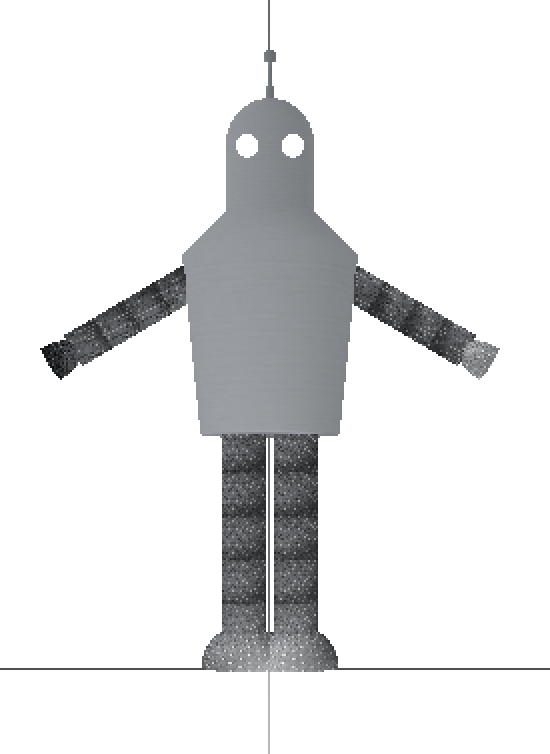
\includegraphics[width=0.3\linewidth]{bender-textura}
	\caption{Bender con texturas aplicadas.}
	\label{fig:bender-textura}
\end{figure}


\newpage
\section{Grafo de escena}

Para facilitar la representación del esquema, cuando introduzcamos en una casilla el nombre de otra clase del esquema en cursiva será equivalente a una flecha de dicha otra clase a la casilla en cuestión.

Añadimos en rojo la inserción de materiales para que se distinga con más facilidad.

\begin{table}[h]
	\centering
	\label{1}
	\begin{tabular}{|c|}
		\hline
		\textbf{Bender Metálico}\\ \hline
		Tras(dist\_lateral, 0, dist\_lineal)\\ \hline
		\textcolor{red}{MaterialMetalico()}\\ \hline
		Esc(0.1, 0.1, 0.1)\\ \hline
		\textit{Cuerpo(true)}\\ \hline
		\textit{CabezaMetálica(true)}\\ \hline
		Tras(0.6, 5.5, 0)\\ \hline
		\textcolor{red}{MaterialMetalicoExtremidad()}\\ \hline
		\textit{Pierna(true)}\\ \hline
		Tras(-1.2, 0, 0)\\ \hline
		\textit{Pierna(true)}\\ \hline
		Tras(0.6, 0, 0)\\ \hline
		\textit{Brazo\_Derecho(true)}\\ \hline
		\textit{Brazo\_Izquierdo(true)}\\ \hline

	\end{tabular}
\end{table}

\begin{table}[h]
	\centering
	\label{2}
	\begin{tabular}{|c|}
		\hline
		\textbf{Cuerpo}\\ \hline
		Esc(2,2,2)\\ \hline
		Tras(0, 3.7, 0)\\ \hline
		\textit{Cilindro\_deforme}\\ \hline

	\end{tabular}
\end{table}



\begin{table}[h!]
	\centering
	\label{4}
	\begin{tabular}{|c|}
		\hline
		\textbf{Cabeza Metálica}\\ \hline
		\textcolor{red}{MaterialMetalico()}\\ \hline
		Tras(0, 9.4, 0)\\ \hline
		Esc(2, 2, 2)\\ \hline
		\textit{Cuello}\\ \hline
		Esc( 0.5, 0.5, 0.5)\\ \hline
		Tras(0, 1.5, 0)\\ \hline
		Rot(15*angulo,0,1,0)\\ \hline
		\textit{Cilindro}\\ \hline
		\textcolor{red}{MaterialOjo()}\\ \hline
		Tras(0,1,0)\\ \hline
		\textit{Ojo}\\ \hline
		Tras(-1, 0, 0)\\ \hline
		\textit{Ojo}\\ \hline
		\textcolor{red}{MaterialMetalico()}\\ \hline
		Tras(0.5, 0, -1)\\ \hline
		Tras(0, 1, 0)\\ \hline
		Esc(0.05, 0.1, 0.1)\\ \hline
		Rot(180,1,0,0)\\ \hline
		\textit{Cono}\\ \hline
		Esc(20,10,10)\\ \hline
		Tras(0, -1.2, 0)\\ \hline
		Esc(0.15, 0.15, 0.15)\\ \hline
		\textit{Esfera}\\ \hline
	\end{tabular}
\end{table}

\begin{table}[h!]
	\centering
	\label{3}
	\begin{tabular}{|c|}
		\hline
		\textbf{Ojo}\\ \hline
		Rot(90, 1, 0, 0)\\ \hline
		Esc(0.25, 0.25, 0.25)\\ \hline
		\textit{Semiesfera}\\ \hline
	\end{tabular}
\end{table}



\begin{table}[h!]
	\centering
	\label{5}
	\begin{tabular}{|c|}
		\hline
		\textbf{Pierna}\\ \hline
		Esc(0.5, 0.5, 0.5)\\ \hline
		Tras(0, -1, 0)\\ \hline
		\textit{Cilindro\_deforme}\\ \hline
		Tras(0,-2,0)\\ \hline
		\textit{Cilindro\_deforme}\\ \hline
		Tras(0,-2,0)\\ \hline
		\textit{Cilindro\_deforme}\\ \hline
		Tras(0,-2,0)\\ \hline
		\textit{Cilindro\_deforme}\\ \hline
		Tras(0,-2,0)\\ \hline
		Esc(2, 2, 2)\\ \hline
		\textit{Semiesfera}\\ \hline
	\end{tabular}
\end{table}

\begin{table}[h!]
	\centering
	\label{6}
	\begin{tabular}{|c|}
		\hline
		\textbf{Brazo\_Derecho}\\ \hline
		Esc(0.4, 0.4, 0.4)\\ \hline
		Tras(5.2, 8, 0)\\ \hline
		Rot(-10*angulo,0,1,0)\\ \hline
		Esc(1, proporción, 1)\\ \hline
		\textit{Cilindro}\\ \hline
		Tras(0, 2*(proporción), 0)\\ \hline
		\textit{Cilindro}\\ \hline
		Tras(0, 2*(proporción), 0)\\ \hline
		\textit{Cilindro}\\ \hline
		Tras(0, 2*(proporción), 0)\\ \hline
		Tras(0, 0.5, 0)\\ \hline
		Rot(180, 1, 0, 0)\\ \hline
		Esc(1, 2, 2)\\ \hline
		\textit{Semiesfera}\\ \hline
	\end{tabular}
\end{table}


\begin{table}[h!]
	\centering
	\label{7}
	\begin{tabular}{|c|}
		\hline
		\textbf{Brazo\_Izquierdo}\\ \hline
		Esc(0.4, 0.4, 0.4)\\ \hline
		Tras(-5.2, 8, 0)\\ \hline
		Rot(10*angulo,0,1,0)\\ \hline
		Esc(1, proporción, 1)\\ \hline
		\textit{Cilindro}\\ \hline
		Tras(0, 2*(proporción), 0)\\ \hline
		\textit{Cilindro}\\ \hline
		Tras(0, 2*(proporción), 0)\\ \hline
		\textit{Cilindro}\\ \hline
		Tras(0, 2*(proporción), 0)\\ \hline
		Tras(0, 0.5, 0)\\ \hline
		Rot(180, 1, 0, 0)\\ \hline
		Esc(1, 2, 2)\\ \hline
		\textit{Semiesfera}\\ \hline
	\end{tabular}
\end{table}

\begin{table}[h!]
	\centering
	\label{8}
	\begin{tabular}{|c|}
		\hline
		\textbf{Semiesfera}\\ \hline
		semiesfera.ply\\ \hline
	\end{tabular}
\end{table}

\begin{table}[h!]
	\centering
	\label{9}
	\begin{tabular}{|c|}
		\hline
		\textbf{Esfera}\\ \hline
		esfera.ply\\ \hline
	\end{tabular}
\end{table}

\begin{table}[h!]
	\centering
	\label{10}
	\begin{tabular}{|c|}
		\hline
		\textbf{Cuello}\\ \hline
		cuello.ply\\ \hline
	\end{tabular}
\end{table}

\begin{table}[h!]
	\centering
	\label{11}
	\begin{tabular}{|c|}
		\hline
		\textbf{Cilindro}\\ \hline
		cilindro.ply\\ \hline
	\end{tabular}
\end{table}


\begin{table}[h!]
	\centering
	\label{12}
	\begin{tabular}{|c|}
		\hline
		\textbf{Cilindro\_deforme}\\ \hline
		cilindro\_deforme.ply\\ \hline
	\end{tabular}
\end{table}



\end{document}